\documentclass[twocolumn]{article}
\usepackage{graphicx}
\usepackage{multicol}
\usepackage{hyperref}

\begin{document}

\begin{center}\Large\textbf{Raw Results}\end{center}

\section{First Runs}

\subsection{Cls}
These are the results from tests run for the poster competition. As you can see in figure \ref{first_cl}, the distributed version of the algorithm finds values that match expectations. The input data is generated from synfast with \emph{Nside32} and one twelfth of the sky is fed into each run. This explains the higher variation in the low bands. This is similar to another graph generated from the original shared version.


\begin{figure}
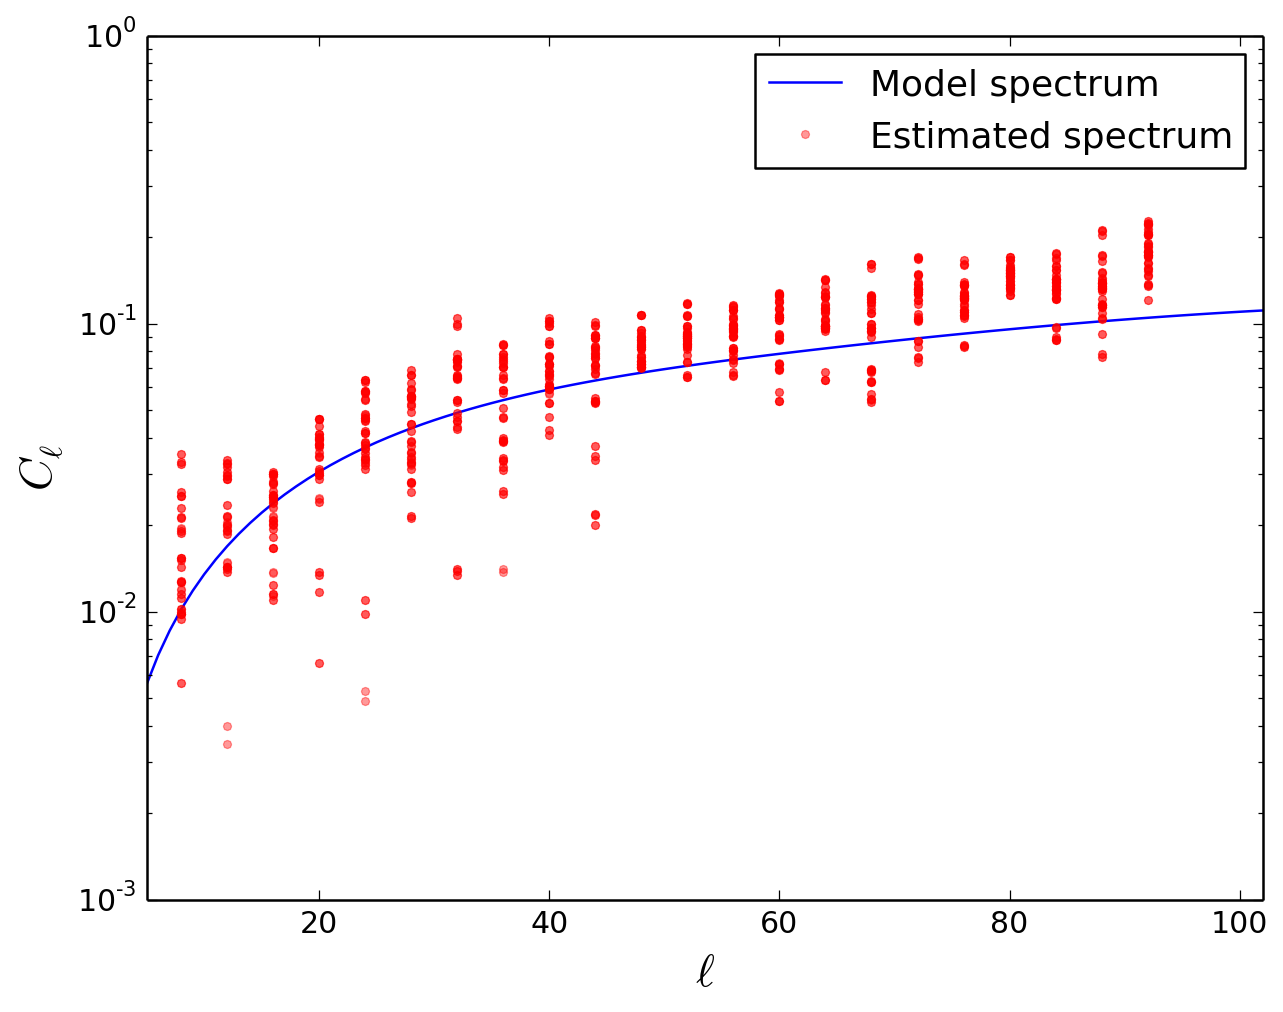
\includegraphics[width=0.9\columnwidth]{figures/cl}
\caption{Cls without KL compression}
\label{first_cl}
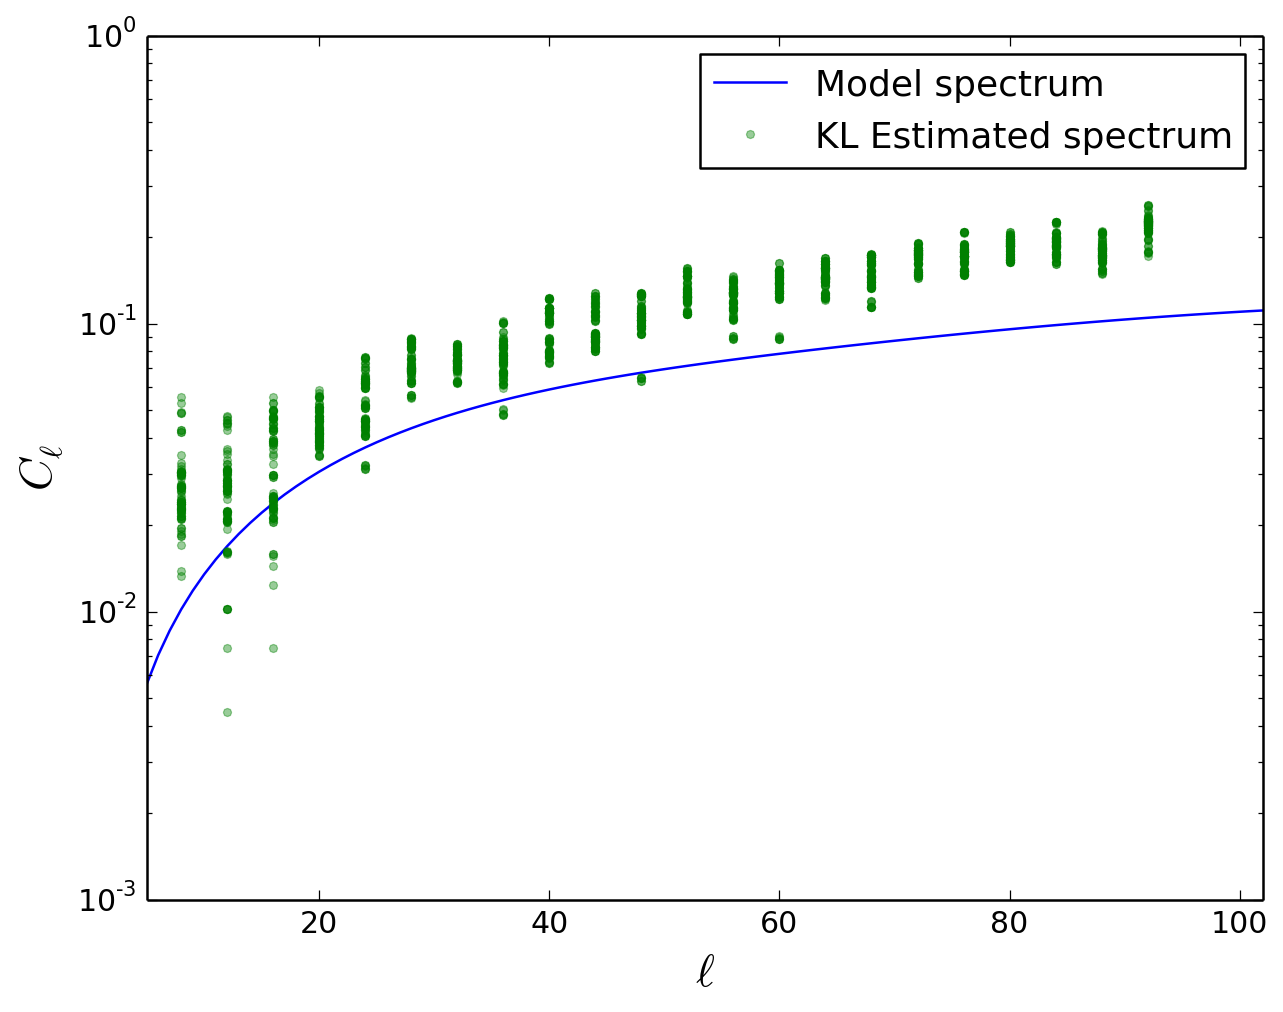
\includegraphics[width=0.9\columnwidth]{figures/kl_cl}
\caption{Cls with KL compression}
\label{first_kl_cl}
\end{figure}

After fixing bugs with KL compression it was possible to do runs to compare the results. In figure \ref{first_kl_cl}, the results do match with the expected line, but with a positive bias. Further investigation is needed to understand the source and nature of the bias.

With the distributed code, it is worth noting that in both runs we were also getting some negative points. This was less the case with KL compression.

\newpage
\subsection{Time and Memory}
To get a better idea of how to run the program with the best performance, the same runs as found cls were used to test timing and memory usage. These runs were done on Taub \url{https://campuscluster.illinois.edu/hardware/#taub}. Using the 24Gb memory nodes with 2 processors each and 6 threads per processor. We can select the number of processors, nodes and MPI processes to create.

\begin{figure}
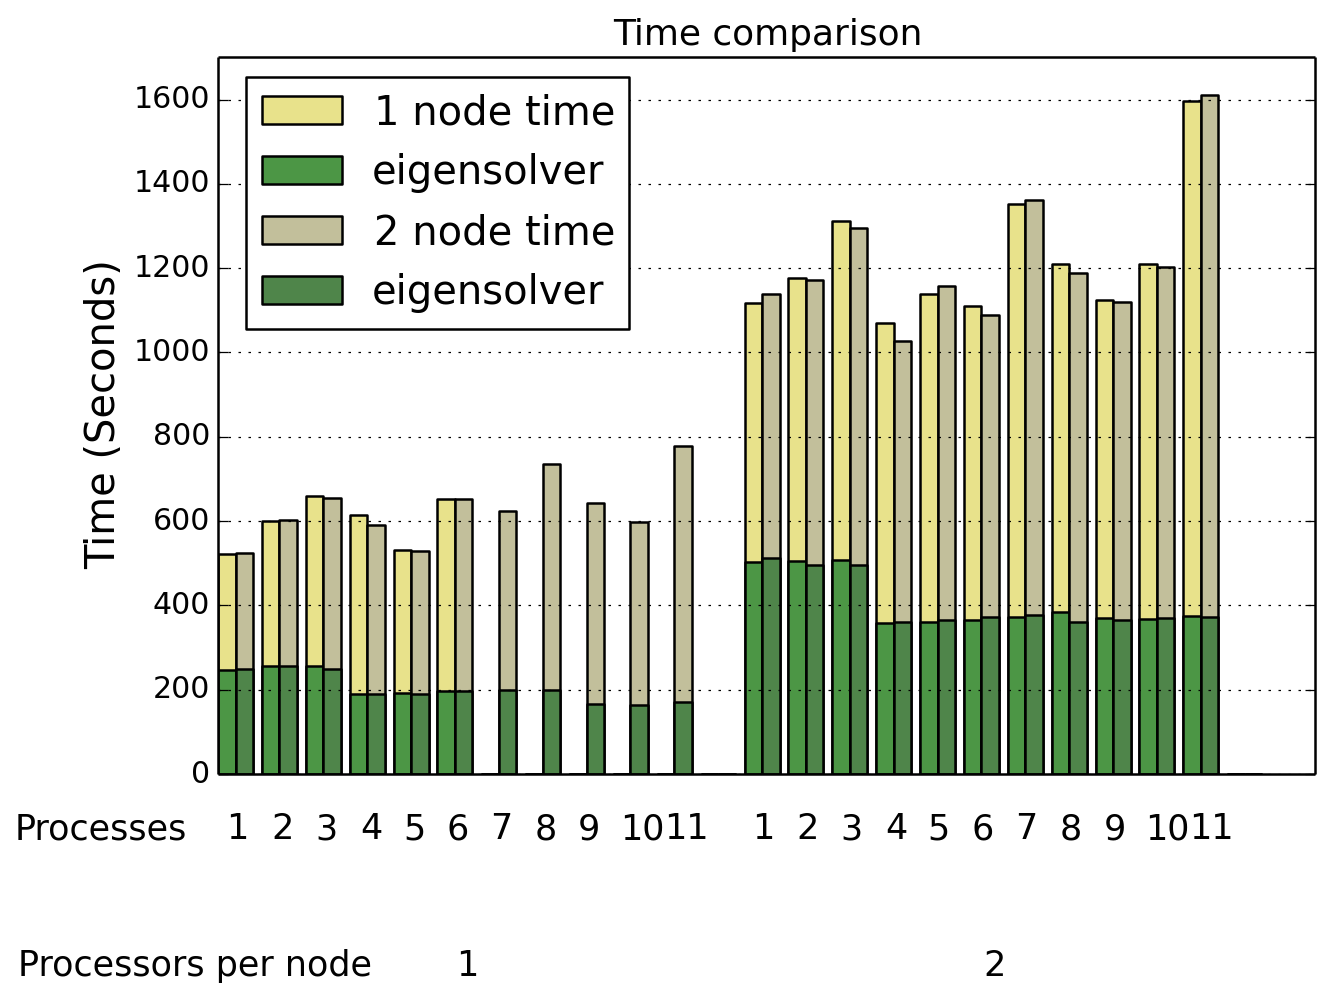
\includegraphics[width=0.9\columnwidth]{figures/node_comp_time}
\caption{Comparison of one vs two nodes, with various number of threads and cores}
\label{node_compare_time}
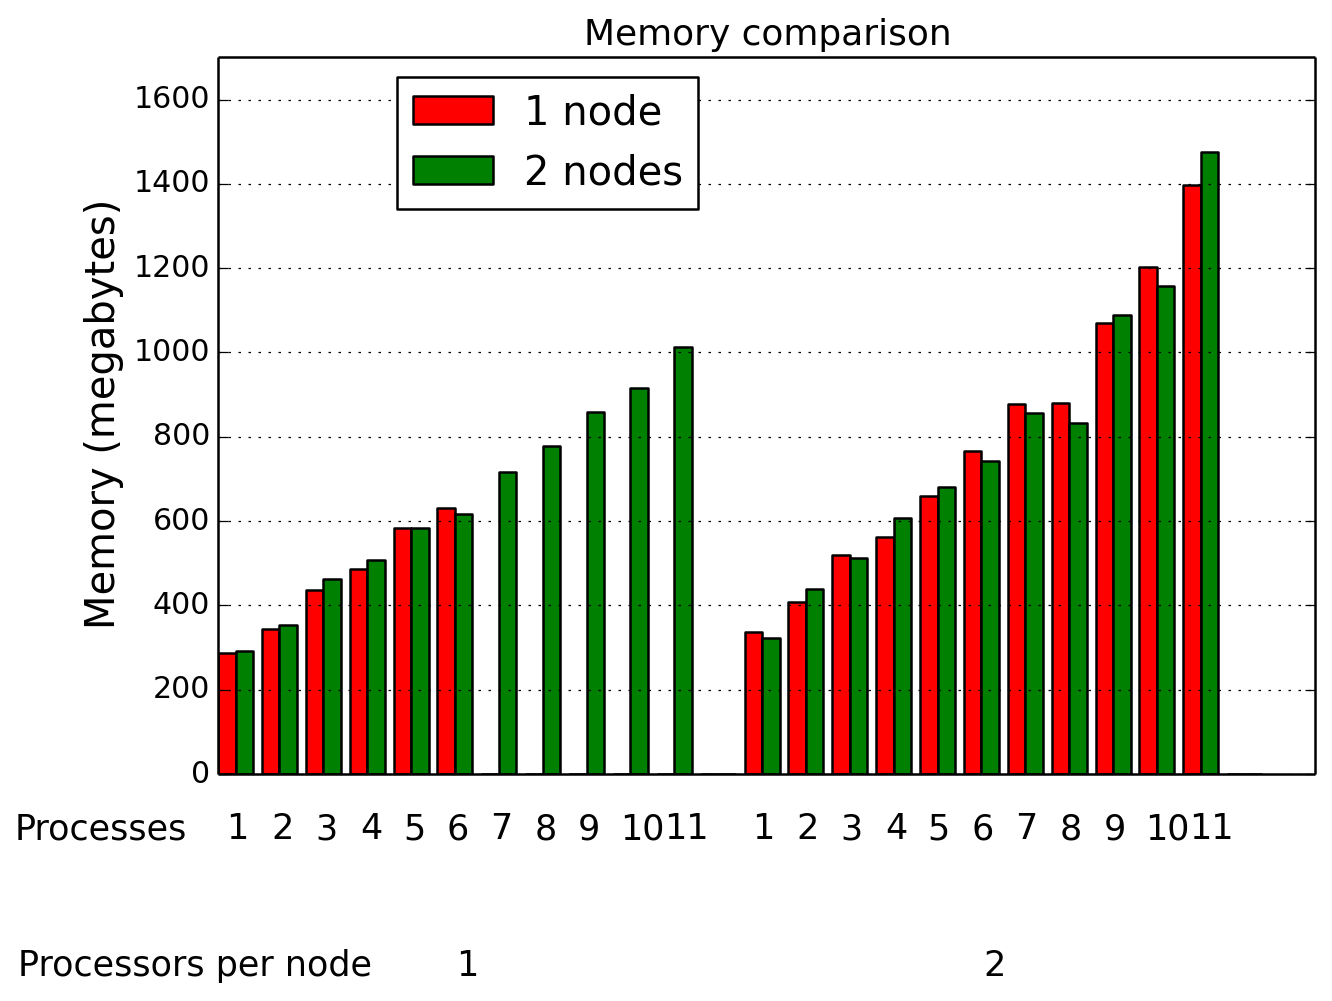
\includegraphics[width=0.9\columnwidth]{figures/node_comp_memory}
\caption{Same comparison but with memory instead of time.}
\label{node_compare_memory}
\end{figure}

The time results in figure \ref{node_compare_time} show that speed decreases with additional processes, although at 4 there is a benefit in the eigensolver. One interesting result is by requesting access to both processors in the node, the time decreases even for one process. One explanation is that cache coherency is slowing it down. It is important to note that \emph{Elemental has thread level parallelism} and is already taking advantage of the available cores.

What is more difficult to explain is why adding another node doesn't effect the time significantly.

Also worth noting is the increasing overhead of having more processes shown in figure \ref{node_compare_memory}.

\subsection{KL compression}
Another topic worth investigating is the effect of changing values for the number of galaxies. When KL compression was run on the current one twelfth sky patch at nside 32 and ngalaxies 1e6, the results were that all of the eigenvalues were lower than a threshold of 1, and thus everything was compressed to nothing. This is not idea, and the synthetic nature of our input data leaves questions as to what is a proper value for ngalaxies, which effects the noise matrix. It is worth asking how the other factors play into this.

In principle the amount of compression would be effected by the initial Cls, nGalaxies, total area of the patch and the number of bins. How these contribute could be analyzed in more depth.

\newpage
Example of the beginning of a run:
\begin{verbatim}
----------------------------------------
Begin Torque Prologue (Sat Aug 16 22:00:47 2014)
Job ID:           1381892.cc-mgmt1.campuscluster.illinois.edu
Username:         amwarren
Group:            mrl_dtrinkle
Job Name:         num_core_compare_nside-32_mpi_nodes-1_cores-2_1b55b13309
Limits:           ncpus=1,neednodes=1:ppn=12:m24G:taub,nodes=1:ppn=12:m24G:taub,walltime=00:28:00
Job Queue:        secondary
Account:          mrl_dtrinkle
Nodes:            taub444
End Torque Prologue
----------------------------------------
mpiexec -verbose -n 1 ./distributed_memory/aps /home/amwarren/aps/data/32_node_compare_7a9f59c4db0592338363-25.fits /home/amwarren/aps/data/32_node_compare_7a9f59c4db0592338363-25.bands num_core_compare_nside-32_mpi_nodes-1_cores-2_1b55b13309
mpiexec: resolve_exe: using absolute path "./distributed_memory/aps".
node  0: name taub444, cpu avail 12
mpiexec: process_start_event: evt 2 task 0 on taub444.
mpiexec: All 1 task (spawn 0) started.
mpiexec: wait_tasks: waiting for taub444.
mpiexec: accept_pmi_conn: cmd=initack pmiid=0.
mpiexec: accept_pmi_conn: rank 0 (spawn 0) checks in.
mpiexec: accept_pmi_conn: cmd=init pmi_version=1 pmi_subversion=1.
\end{verbatim}

\end{document}